% \documentclass{article}
% \usepackage{arxiv}

% \usepackage[utf8]{inputenc}
% \usepackage[english, russian]{babel}
% \usepackage[T1]{fontenc}
% \usepackage{url}
% \usepackage{booktabs}
% \usepackage{amsfonts}
% \usepackage{nicefrac}
% \usepackage{microtype}
% \usepackage{lipsum}
% \usepackage{graphicx}
% \usepackage{natbib}
% \usepackage{doi}
% \usepackage{amsmath}
% \usepackage{hyperref}
% \usepackage{caption}
% \DeclareMathOperator*{\argmax}{arg\,max}
% \DeclareMathOperator*{\argmin}{arg\,min}
\documentclass[a4paper,12pt]{article}

\usepackage[T2A]{fontenc}
\usepackage[utf8]{inputenc}
\usepackage[english,russian]{babel}
\usepackage{tikz}                % для создания иллюстраций
\usepackage{pgfplots}            % для вывода графиков функций
\usepackage{geometry}		 % для настройки размера полей
\usepackage{indentfirst}         % для отступа в первом абзаце секции
\def\code#1{\texttt{#1}}
\usepackage{float}

\geometry{a4paper,left=30mm,top=20mm,bottom=20mm,right=15mm}

\setcounter{secnumdepth}{0}      % отключаем нумерацию секций

\usepgfplotslibrary{fillbetween} % для изображения областей на графиках
%\usepackage{graphics}
\usepackage{graphicx}
\usepackage{amsmath}
\usepackage{amsthm}
\usepackage{wasysym}
\usepackage{amssymb}
\usepackage{hyperref}
\usepackage{url}
\usepackage{booktabs}
\usepackage{amsfonts}
\usepackage{nicefrac}
\usepackage{microtype}
\usepackage{natbib}
\usepackage{doi}
\usepackage{caption}
\DeclareMathOperator*{\argmax}{arg\,max}
\DeclareMathOperator*{\argmin}{arg\,min}
\linespread{1.5}
\hypersetup{
    colorlinks=true,
    linkcolor=black,
    filecolor=magenta,      
    urlcolor=blue
    }

\usepackage{algorithm,algcompatible,amsmath}
\algnewcommand\INPUT{\item[\textbf{Ввод:}]}%
\algnewcommand\OUTPUT{\item[\textbf{Вывод:}]}%
\algnewcommand\COMM{\item[Комментарий:]}%

\title{Выпускная квалификационная работа}

\author{ Валентин А. Абрамов \\
	Факультет вычислительной математики и кибернетики\\
	МГУ имени М. В. Ломоносова\\
	%% \AND
	%% Coauthor \\
	%% Affiliation \\
	%% Address \\
	%% \texttt{email} \\
	%% \And
	%% Coauthor \\
	%% Affiliation \\
	%% Address \\
	%% \texttt{email} \\
	%% \And
	%% Coauthor \\
	%% Affiliation \\
	%% Address \\
	%% \texttt{email} \\
}
\date{}

% \renewcommand{\shorttitle}{\textit{arXiv} Template}
% \renewcommand{\abstractname}{Аннотация}
%%% Add PDF metadata to help others organize their library
%%% Once the PDF is generated, you can check the metadata with
%%% $ pdfinfo template.pdf
% \hypersetup{
% pdftitle={A template for the arxiv style},
% pdfsubject={q-bio.NC, q-bio.QM},
% pdfauthor={David S.~Hippocampus, Elias D.~Striatum},
% pdfkeywords={First keyword, Second keyword, More},
% }


\begin{document}

\begin{titlepage}
\begin{center}
    Московский государственный университет имени М. В. Ломоносова

    \bigskip
    
\includegraphics[width=50mm]{msu.eps}

    \bigskip
    Факультет Вычислительной Математики и Кибернетики\\
    Кафедра Математических Методов Прогнозирования\\[10mm]

    \textsf{\large\bfseries
         Выпускная квалификационная работа\\[10mm]
        <<Эволюционный алгоритм подбора гиперпараметров моделей>>
    }\\[10mm]

    \begin{flushright}
        \parbox{0.5\textwidth}{
            Выполнил:\\
            студент 4 курса 417 группы\\
            \emph{Абрамов Валентин Андреевич}\\[5mm]
            Научный руководитель:\\
            к.ф.-м.н.\\
            \emph{Китов Виктор Владимирович}
        }
    \end{flushright}

    \vspace{\fill}
    Москва
    
    2024
\end{center}
\end{titlepage}
% Автоматически генерируем оглавление на отдельной странице
\setcounter{page}{2}
\tableofcontents
\newpage
\section{Введение}

В последние годы машинное обучение стало одной из самых активно 
развивающихся областей в информационных технологиях. Чтобы достичь 
оптимального качества моделей машинного обучения, необходимо правильно 
настроить конфигурацию этих моделей, то есть тщательно подобрать 
наилучшие гиперпараметры для этих моделей.
Примерами гиперпараметров выступает число K в методе K ближайших 
соседей, сила регуляризации в линейных моделях, число слоев и нейронов на 
каждом слое в нейронных сетях и т.д.

Гиперпараметры являются важными параметрами моделей машинного 
обучения, которые не могут быть настроены по обучающей выборке 
градиентными методами — для этого необходимо оценивать точность модели 
на отдельной валидационной выборке либо перебирая всевозможные 
гиперпараметры вручную (что требует экспертизы и занимает много времени), 
либо используя автоматические методы безградиентной оптимизации. 
Простейшие методы автоматического выбора гиперпараметров, такие, как 
перебор по равномерной сетке или случайный поиск, могут быть 
неэффективными или требовать значительных вычислительных ресурсов, 
поэтому вместо них используют более сложные алгоритмы, например, 
эволюционные [1].

Работа состоит из двух частей: в первой предлагается новое исследование -- новые алгоритмы оптимизации гиперпараметров, во второй -- модификация алгоритма DEHB [2]. Вторая часть была представлена на конференции ИТиММ-2024 в РЭУ имени Г.В. Плеханова.

\section{Часть 1}
В данной части рассматриваются существующие методы оптимизации гиперпараметров, работающие как с непрерывными, так и с категориальными параметрами. Предлагается новый метод, проводятся эксперименты для сравнения результатов работы нового метода с другими.

\section{Обзор литературы}

Гиперпараметрическая оптимизация — большая и перспективная область исследований. В данный момент в исследованиях поднимаются вопросы переобучения гиперпараметров на валидационную выборку и параллелизации алгоритмов [3]. Для глубоких нейронных сетей также необходимо подбирать гиперпараметры, такие, как число слоев, скорость обучения и даже связи между слоями [4].

Задача автоматического подбора гиперпараметров активно исследуется. Широко используемые методы перебора значений по сетке и случайного поиска имеют низкую вычислительную эффективность, поскольку не учитывают информацию о качестве ранее протестированных конфигураций (наборов гиперпараметров) для генерации новых конфигураций. 

В 2011 году был создан подход SMBO — последовательная оптимизация, основанная на суррогатной функции, то есть функции, приближающей целевую оптимизируемую функцию, но быструю для расчета [5]. В качестве суррогатной функции изначально брали гауссовские процессы, но они подходят не для всех задач, так как предназначены только для непрерывных гиперпараметров [6]. 

На данный момент одним из лучших методов автоматического подбора гиперпараметров является метод TPE, основанный на байесовском подходе [7]. Также существуют методы, основанные на подходе SMBO, такие, как SMAC, использующий случайный лес в качестве суррогата, или модели, использующие суррогат на основе гауссовских процессов [5, 6, 8, 9].

При оптимизации гиперпараметров также используются эволюционные алгоритмы, так как они позволяют оптимизировать любые функции за счет интеллектуального перебора значений, основанного на таких идеях эволюции, как мутация, скрещивание, селекция и естественный отбор [10, 11]. 

Хорошее качество обеспечивает метод Successive Halving (SH)  – он позволяет найти лучший набор гиперпараметров в условиях ограниченности вычислительных мощностей [12]. На основе SH созданы алгоритмы HyperBand, автоматически выделяющий ресурсы для нескольких запусков SH, BOHB, добавляющий в HyperBand суррогат на основе подходов TPE, и DEHB, добавляющий в HyperBand идею дифференциальной эволюции [2, 13, 14].

\section{Постановка задачи}
Задача гиперпараметрической оптимизации состоит в том, чтобы имея обучающую выборку $X \in \mathbb{R}^{N\times d}, y \in \mathbb{R}^{N}$, пространство гиперпараметров $\Theta \in \mathbb{R}^k$, модель $f(\theta): \mathbb{R}^{d} \to \mathbb{R},\ \theta \in \Theta$, $f \in \mathbb{H}$ и функцию ошибок $\mathcal{L}(f, X, y): \mathbb{H} \times \mathbb{R}^{N\times d} \times \mathbb{R}^{N} \to \mathbb{R}$, найти $\theta^*$ такую, что выполнено
$$\theta^* = \argmin_{\theta} \mathcal{L}(f(\theta), X, y)$$
Таким образом, зная модель $f$, пространство гиперпараметров $\Theta$, набор данных $X, y$ и функцию ошибок $\mathcal{L}$, необходимо найти набор гиперпараметров $\theta^*$, при котором значение функции ошибок $\mathcal{L}$ наименьшее при обучении модели $f$ на данных $X, y$.

Предполагается, что набор гиперпараметров состоит из непрерывных и категориальных переменных, функция $\mathcal{L}$ имеет бюджет вычислений. Им может быть ограничение на максимальное число итераций при обучении нейронной сети, количество деревьев в случайном лесе и градиентном бустинге и т. п.


\section{Существующие методы}
\subsection{Поиск по сетке}
Поиск по сетке работает следующим образом:
\begin{enumerate}
    \item Задаются наборы значений параметров.
    \item Для каждой комбинации параметров вычисляется значение целевой функции.
\end{enumerate}

У этого подхода есть множество известных проблем:
\begin{enumerate}
    \item Необходимость выбора сетки значений вручную.
    \item Медленное время работы.
    \item В случае, когда один гиперпараметр влияет сильнее, чем другие, перебор неэффективен из-за многократного использования одного значения существенного гиперпараметра.
\end{enumerate}


\subsection{Случайный поиск}
Случайный поиск работает следующим образом:
\begin{enumerate}
    \item Наборы параметров случайно сэмплируются из некоторого распределения.
    \item Для каждого набора параметров вычисляется значение целевой функции.
\end{enumerate}

Случайный поиск избавлен от проблем поиска по сетке, но также имеет недостатки:
\begin{enumerate}
    \item Перебор не использует вычисленные значения функции ошибок.
    \item Поиск ненаправленный, то есть наборы гиперпараметров сэмплируются полностью случайно.
\end{enumerate}

\subsection{Эволюционный алгоритм}
Для краткости будем называть наборы гиперпараметров кандидатами. Классический эволюционный алгоритм работает следующим образом:
\begin{enumerate}
    \item Создается набор кандидатов размера $N$, называемый популяцией.
    \item Повторяются следующие действия:
    \begin{enumerate}
        \item Вычисляется значение оптимизируемой функции для каждого кандидата.
        \item Отбирается $M$ лучших по значению функции кандидатов.
        \item Создаются новые $N - M$ кандидатов путем скрещивания $2$ случайных кандидатов из $M$ лучших и мутации.
    \end{enumerate}
\end{enumerate}

Начальные кандидаты сэмплируются из равномерного распределения или из распределений, выбираемых пользователем.
В качестве операции скрещивания используется биномиальное скрещивание -- выбор значения параметра одного из кандидатов-родителей с вероятностью $0.5$. Мутация -- замена параметра на случайное значение с вероятностью $p$. В таком подходе $N, M, p$ -- параметры эволюционного алгоритма, эволюция происходит, пока не будет достигнуто определенное число итераций, время работы или пока лучшее достигнутое значение оптимизируемой функции не перестанет изменяться в течение некоторого заранее определенного числа итераций. Результат работы такого алгоритма - лучший кандидат по значению функции. 

\begin{algorithm}[H]
    \caption{Эволюционный алгоритм}\label{alg:evo}
  \begin{algorithmic}[1]
    \INPUT $N$ -- размер популяции, $M$ -- количество выживших на каждом этапе, $p$ -- вероятность мутации, $f$ -- оптимизируемая функция, распределения гиперпараметров $p_{j}(\theta) (j = 1,\dots,d)$, условие остановки.
    \OUTPUT $\theta^*$ -- набор гиперпараметров с наименьшим значением $f$ из всех обработанных наборов.
    \STATE $\Theta \gets \{\theta^k\ |\ k = 1,\dots,N\},\ \theta^k_j \sim p_j(\theta)\ \forall j = 1,\dots,d$
    \WHILE{<не выполено условие остановки>}
        \STATE $F \gets \{f(\theta)\ |\ \forall \theta \in \Theta\}$
        \STATE $\Theta \gets \{M \text{ лучших по значению } f \text{ наборов гиперпараметров}\}$
        \STATE $\Theta_{new} \gets \emptyset$
        \WHILE{$|\Theta_{new}| < N - M$}
            \STATE $\theta_1, \theta_2 \gets \Theta$ -- случайный выбор без возвращения двух родителей
            \STATE $\theta_{new} \gets Crossover(\theta_1, \theta_2)$ -- скрещивание
            \STATE $\theta_{new} \gets Mutation(\theta_{new}, p, p_{j}(\theta) (j = 1,\dots,d))$ -- мутация
            \STATE $\Theta_{new} \gets \Theta_{new} \cup \{\theta_{new}\} $ -- мутация
        \ENDWHILE
        \STATE $\Theta \gets \Theta \cup \Theta_{new}$
    \ENDWHILE
  \end{algorithmic}

\end{algorithm}

Перечислим слабые стороны эволюционных алгоритмов:
\begin{enumerate}
    \item Алгоритмы требуют многократного вычисления функции $f$, которая может вычисляться очень долго при обучении моделей.
    \item При мутации не учитывается положительный опыт, есть риск ухудшения набора гиперпараметров при неудачном сэмплировании.
\end{enumerate}

\newpage

\subsection{Successive Halving}

\begin{figure}[h]
    \centering
    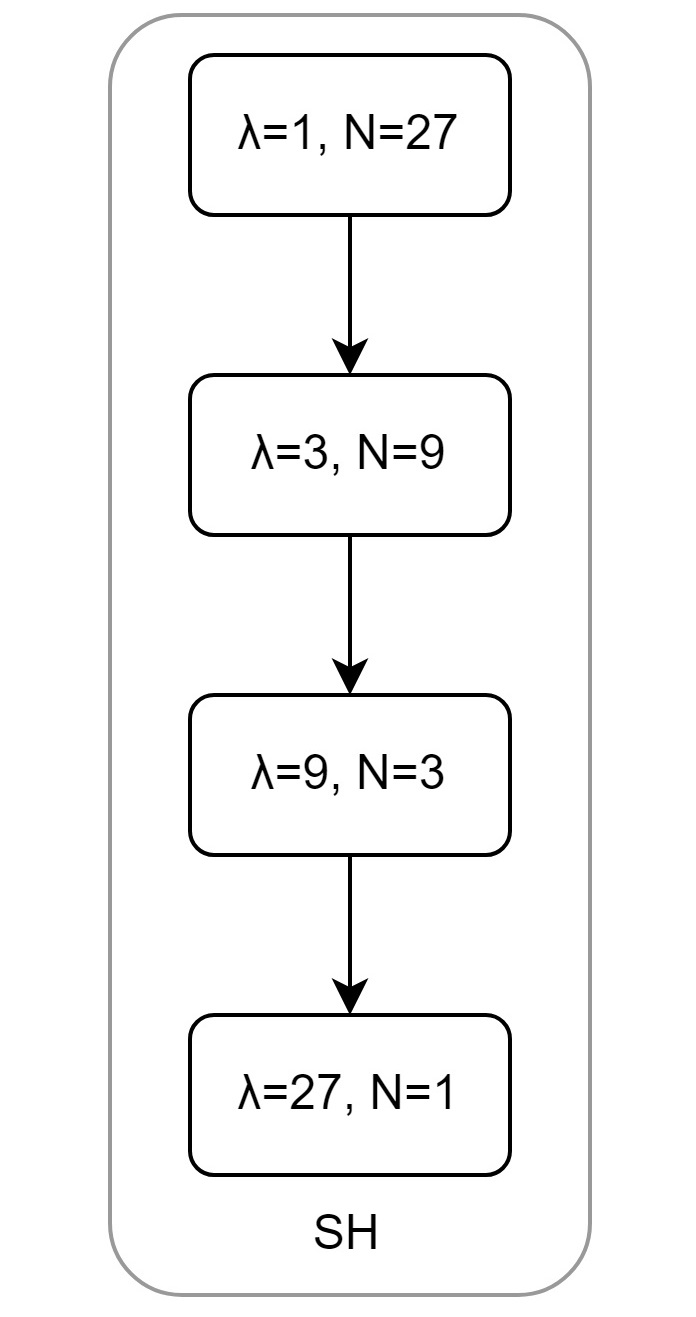
\includegraphics[height=8cm]{SH.jpg}
    \caption{Схема работы Successive Halving, $\lambda_{min}=1,\lambda_{max}=27, \eta=3$}
    \label{fig:sh}
\end{figure}

Successive Halving (рис. \ref{fig:sh}) -- алгоритм подбора гиперпараметров, подразумевающий наличие бюджета вычислений, то есть целевую функцию $f$ можно вычислить с фиксированным бюджетом [12]. Например, можно ограничить количество итераций обучения нейросети или ограничить число деревьев при обучении случайного леса. 
У алгоритма есть три гиперпараметра: минимальный бюджет $\lambda_{min}$, максимальный бюджет $\lambda_{max}$, и $\eta$ -- параметр шкалирования. На первой итерации из равномерного распределения сэмплируются $N_1$ кандидатов, для них вычисляется функция $f$ с бюджетом $\lambda_1 = \lambda_{min}$. На второй итерации берутся $N_2 = N_1/\eta$ лучших кандидатов, для них вычисляется $f$ с бюджетом $\lambda_2 = \eta\lambda_1$. На i-ой итерации функция $f$ вычисляется для $N_i = N_1/\eta^{i - 1}$ лучших кандидатов с шага $i - 1$ с бюджетом $\lambda_i = \eta^{i - 1}\lambda_1$. $\lambda_1$ и $N_1$ выбираются так, чтобы бюджет вычислений на последней итерации был равен 1 для единственного кандидата.  Таким образом, алгоритм работает как случайный поиск, который выделяет больше вычислительных ресурсов перспективным кандидатам и отсекает тех, кто при низком бюджете показывает себя хуже остальных.

\newpage

\begin{algorithm}[H]
    \caption{Successive Halving}\label{alg:sh}
  \begin{algorithmic}[1]
    \INPUT Бюджеты вычислений $\lambda_{min}, \lambda_{max}$, параметр шкалирования $\eta$, максимальное число наборов $N_{max}$, функция ошибок $f(\theta, \lambda)$, распределения гиперпараметров $p_{j}(\theta) (j = 1,\dots,d)$.
    \OUTPUT $\theta^*$ -- набор гиперпараметров с наименьшим значением $f(\cdot, \lambda_{max})$ из всех обработанных наборов.
    \STATE $s \gets \lfloor \log_{\eta} \frac{\lambda_{max}}{\lambda_{min}} \rfloor + 1$
    \STATE $\lambda_{1} \gets \lambda_{min}$
    \STATE $N_{1} \gets N_{max}$
    \STATE $\Theta \gets \{\theta^k\ |\ k = 1,\dots,N_{max}\},\ \theta^k_j \sim p_j(\theta)\ \forall j = 1,\dots,d$
    \FOR{$k = 1,\dots,s$}
        \STATE $F \gets \{f(\theta, \lambda_k)\ |\ \forall \theta \in \Theta\}$
        \STATE $\Theta \gets \{\lfloor \frac{N_k}{\eta} \rfloor \text{ лучших по значению } f(\cdot, \lambda_k) \text{ наборов гиперпараметров}\}$
        \STATE $N_{k+1} \gets \lfloor \frac{N_k}{\eta} \rfloor$
        \STATE $\lambda_{k+1} \gets \lambda_k\eta$
    \ENDFOR
  \end{algorithmic}

\end{algorithm}

\subsection{HyperBand}

\begin{figure}[h]
    \centering
    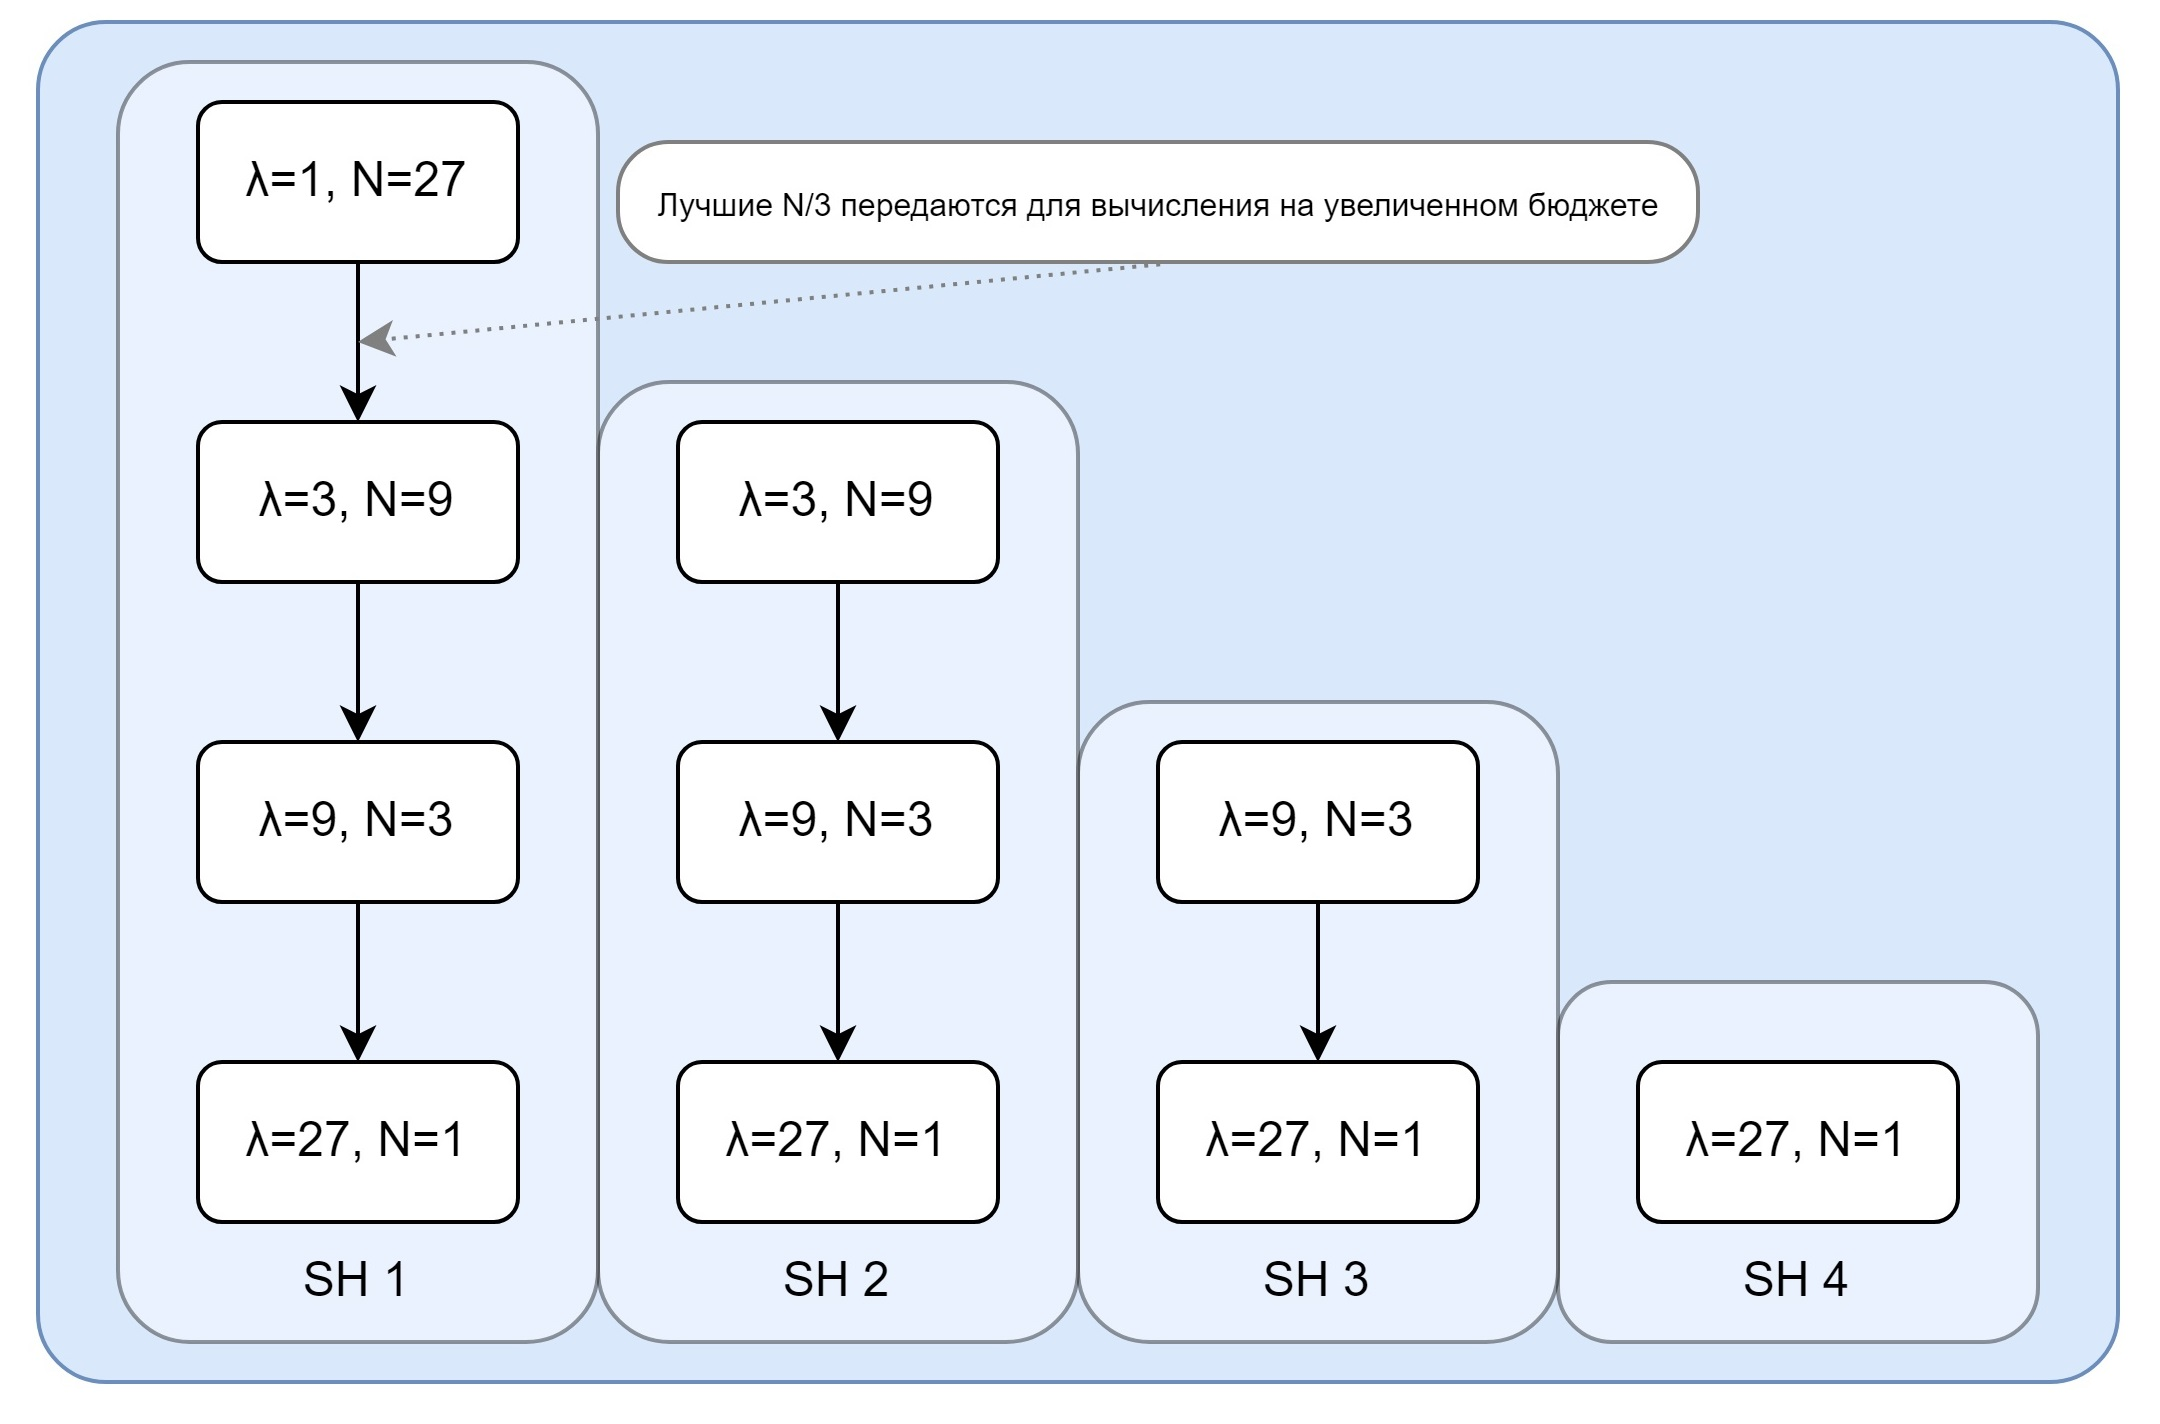
\includegraphics[height=8cm]{HB.jpg}
    \caption{Схема работы HyperBand, $\lambda_{min}=1,\lambda_{max}=27, \eta=3$}
    \label{fig:hb}
\end{figure}

HyperBand (рис. \ref{fig:hb}) расширяет идеи SH -- производится несколько запусков SH с различными значениями $\lambda_{min}$ [13]. Для каждого нового запуска увеличивается минимальный бюджет. Таким образом, функции $f$, которые долго сходятся, проверяются для случайных инициализаций и с низким бюджетом, и с высоким. 

\begin{algorithm}[H]
    \caption{HyperBand}\label{alg:hb}
  \begin{algorithmic}[1]
    \INPUT Бюджеты вычислений $\lambda_{min}, \lambda_{max}$, параметр шкалирования $\eta$, максимальное число наборов $N_{max}$, функция ошибок $f(\theta, \lambda)$, распределения гиперпараметров $p_{j}(\theta) (j = 1,\dots,d)$.
    \OUTPUT $\theta^*$ -- набор гиперпараметров с наименьшим значением $f(\cdot, \lambda_{max})$ из всех обработанных наборов. Возвращаем лучшую $\theta^*$
    \STATE $s_{max} \gets \lfloor \log_{\eta} \frac{\lambda_{max}}{\lambda_{min}} \rfloor + 1$
    \STATE $\Theta^* \gets \emptyset$ -- множество оптимальных значений для каждого запуска SH.
    \FOR{$s = 0,\dots,s_{max}$}
        \STATE $\hat{\lambda}_{min} \gets \lambda_{min}\eta^{s}$
        \STATE $\hat{N}_{max} \gets \frac{N_{max}}{\eta^{s}}$
        \STATE $\theta^* \gets SuccessiveHalving(\hat{\lambda}_{min}, \lambda_{max}, \eta, \hat{N}_{max}, f, p_{j}(\theta) (j = 1,\dots,d))$
        \STATE $\Theta^* \gets \Theta^* \cup \{\theta^*\}$
    \ENDFOR
  \end{algorithmic}

\end{algorithm}

Параметры $\lambda_{min},\lambda_{max}$ и $N_{max}$ обычно выбираются из следующих соображений: $\lambda_{min}$ выбирается как минимальный бюджет, при котором имеется смысл вычислять оптимизируемую функцию, $\lambda_{max}$ выбирается как максимальный приемлемый бюджет вычислений, $N_{max}$ выбирается равным $\lambda_{max}$ (так на последней итерации SH останется ровно один набор гиперпараметров).

У SH и HyperBand есть следующие слабые стороны:
\begin{enumerate}
    \item Алгоритмы полностью полагаются на случайное сэмплирование.
    \item Алгоритмы не учитывают положительный и отрицательный опыт при генерации новых кандидатов.
    \item Не всегда гиперпараметры, отсеянные при низком бюджете, являются плохими при высоком.
\end{enumerate}

\subsection{Tree-structured Parzen estimator}
Данный метод в начале работает как случайный поиск, а после оценки некоторого заранее заданного числа значений функции начинает действовать по следующему алгоритму [7]:
\begin{enumerate}
    \item Набор параметров строится следующим образом. Для каждого параметра выполняются действия:
    \begin{enumerate}
        \item На основе значений целевой функции строятся распределения $l_{par}(x)$ лучших значений параметра и $g_{par}(x)$ худших значений параметра.
        \item Сэмплируются новые значения параметра из $l_{par}(x)$.
        \item Значение параметра выбирается на основе полученных распределений лучших и худших как значение, максимизирующее Expected Improvement: $EI = \frac{l_{par}(x)}{g_{par}(x)}$
    \end{enumerate}
    \item Для полученного набора параметров вычисляется значение целевой функции.
    
\end{enumerate}

Этот алгоритм является одним из самых технически продвинутых на данный момент, но у него также есть слабые стороны:
\begin{enumerate}
    \item Для корректного построения распределений параметров $l_{par}(x)$ и $g_{par}(x)$ необходим ``прогрев'' случайным поиском в течение большого числа итераций.
    \item Алгоритм требует многократного вычисления функции $f$, которая может вычисляться очень долго при обучении моделей.
\end{enumerate}

Стоит сказать, что есть и другие методы, например, основанные на байесовской оптимизации, но они работают только с непрерывными гиперпараметрами, а на данный момент у моделей машинного обучения достаточно большая часть параметров дискретна или имеет только строковое представление.

\newpage

\section{Предлагаемый метод: EvoHyperBand}
Предлагается объединить Successive Halving и эволюционный алгоритм следующим образом: на этапе перехода между уровнями бюджета $\lambda_i$ и $\lambda_{i+1} = \eta\lambda_i$ брать $\frac{N_i}{\nu\eta}$ лучших кандидатов, а оставшиеся $\frac{N_i}{\eta} - \frac{N_i}{\nu\eta}$ получать скрещиванием и мутацией лучших, как в эволюционном алгоритме. Таким образом, получим метод, который:
\begin{enumerate}
    \item Не будет полностью полагаться на случайное сэмплирование в начале итерации Successive Halving.
    \item Благодаря мутации на высоких уровнях бюджета возможно возвращение некоторых значений параметров, которые были  на низких уровнях бюджета.
    \item Перебор будет более широким за счет дополнительной случайности при мутации.
\end{enumerate}

\begin{algorithm}[H]
    \caption{Модификация Successive Halving: \textbf{EvoSH}}\label{alg:esh}
  \begin{algorithmic}[1]
    \INPUT Бюджеты вычислений $\lambda_{min}, \lambda_{max}$, параметр шкалирования $\eta$, \textbf{параметр доли $\nu$, вероятность мутации $p$}, максимальное число наборов $N_{max}$, функция ошибок $f(\theta, \lambda)$, распределения гиперпараметров $p_{j}(\theta) (j = 1,\dots,d)$.
    \OUTPUT $\theta^*$ -- набор гиперпараметров с наименьшим значением $f(\cdot, \lambda_{max})$ из всех обработанных наборов.
    \STATE $s \gets \lfloor \log_{\eta} \frac{\lambda_{max}}{\lambda_{min}} \rfloor + 1$
    \STATE $\lambda_{1} \gets \lambda_{min}$
    \STATE $N_{1} \gets N_{max}$
    \STATE $\Theta \gets \{\theta^k\ |\ k = 1,\dots,N_{max}\},\ \theta^k_j \sim p_j(\theta)\ \forall j = 1,\dots,d$
    \FOR{$k = 1,\dots,s$}
        \STATE $F \gets \{f(\theta, \lambda_k)\ |\ \forall \theta \in \Theta\}$
        \STATE $\Theta \gets \{\lfloor \frac{N_k}{\eta\nu} \rfloor \text{ лучших по значению } f(\cdot, \lambda_k) \text{ наборов гиперпараметров}\}$
        \STATE $\Theta_{new} \gets \emptyset$
        \WHILE{$|\Theta_{new}| < \lfloor \frac{N_k}{\eta} \rfloor - \lfloor \frac{N_k}{\eta\nu} \rfloor$}
            \STATE $\theta_1, \theta_2 \gets \Theta$ -- случайный выбор без возвращения двух родителей
            \STATE $\theta_{new} \gets Crossover(\theta_1, \theta_2)$ -- скрещивание
            \STATE $\theta_{new} \gets Mutation(\theta_{new}, p, p_{j}(\theta) (j = 1,\dots,d))$ -- мутация (сэмплирование параметров из заданных распределений с вероятностью p)
            \STATE $\Theta_{new} \gets \Theta_{new} \cup \{\theta_{new}\} $
        \ENDWHILE
        \STATE $\Theta \gets \Theta \cup \Theta_{new}$
        \STATE $N_{k+1} \gets \lfloor \frac{N_k}{\eta} \rfloor$
        \STATE $\lambda_{k+1} \gets \lambda_k\eta$
    \ENDFOR
  \end{algorithmic}

\end{algorithm}


\begin{algorithm}[H]
    \caption{EvoHyperBand}\label{alg:ehb}
  \begin{algorithmic}[1]
    \INPUT Бюджеты вычислений $\lambda_{min}, \lambda_{max}$, параметр шкалирования $\eta$, \textbf{параметр доли $\nu$, вероятность мутации $p$} максимальное число наборов $N_{max}$, функция ошибок $f(\theta, \lambda)$, распределения гиперпараметров $p_{j}(\theta) (j = 1,\dots,d)$.
    \OUTPUT $\theta^*$ -- набор гиперпараметров с наименьшим значением $f(\cdot, \lambda_{max})$ из всех обработанных наборов.
    \STATE $s_{max} \gets \lfloor \log_{\eta} \frac{\lambda_{max}}{\lambda_{min}} \rfloor + 1$
    \STATE $\Theta^* \gets \emptyset$ -- множество оптимальных значений для каждого запуска SH.
    \FOR{$s = 0,\dots,s_{max}$}
        \STATE $\hat{\lambda}_{min} \gets \lambda_{min}\eta^{s}$
        \STATE $\hat{N}_{max} \gets \frac{N_{max}}{\eta^{s}}$
        \STATE $\theta^* \gets EvoSH(\hat{\lambda}_{min}, \lambda_{max}, \eta, \nu, p, \hat{N}_{max}, f, p_{j}(\theta) (j = 1,\dots,d))$
        \STATE $\Theta^* \gets \Theta^* \cup \{\theta^*\}$
    \ENDFOR
  \end{algorithmic}

\end{algorithm}

Данную модификацию Successive Halving будем запускать в режиме HyperBand и назовем данный алгоритм EvoHyperBand. Эксперименты показали, что для большинства задач оптимальное значение $\nu=2$. 

\section{Предлагаемый метод: EvoHyperBandMut}
У предложенного метода остается проблема эволюционных алгоритмов: при мутации никак не учитывается предыдущий положительный опыт, то есть сэмплирование при мутации полностью случайное.

Предлагается модифицировать мутацию следующим образом:
\begin{itemize}
    \item При переходе с первого уровня первой итерации Successive Halving в мутации происходит сэмплирование из заданных пользователем распределений (как в эволюционном алгоритме выше).
    \item Все наборы гиперпараметров и значения целевой функции на них сохраняются.
    \item После каждой итерации Successive Halving для каждого оптимизируемого гиперпараметра $par$ строится оценка плотности $\hat{p}_{par}$.
    \begin{itemize}
        \item Для непрерывных -- ядровая оценка плотности суммой гауссиан с параметром $bandwidth = n^{-\frac{1}{5}}$ ($n$ -- количество точек), для категориальных -- частотная оценка. Параметр $bandwidth$ взят из сборника [15].
        \item Плотность оценивается по наборам гиперпараметров, для которых значение целевой функции больше некоторого квантиля $\chi$ ($\chi$ брался равным 0.5).
    \end{itemize}
    \item При мутации каждый мутируемый параметр сэмплируется из плотности $\hat{p}_{par}$ с вероятностью $p$ (параметр метода).
\end{itemize}

Предполагается, что такая модификация позволит получать лучшие наборы гиперпараметров в результате мутации, назовем ее EvoHyperBandMut.

\begin{algorithm}[H]
    \caption{EvoHyperBandMut}\label{alg:ehbmut}
  \begin{algorithmic}[1]
    \INPUT Бюджеты вычислений $\lambda_{min}, \lambda_{max}$, параметр шкалирования $\eta$, \textbf{параметр доли $\nu$, параметр квантиля $\chi$, вероятность мутации $p$}, максимальное число наборов $N_{max}$, функция ошибок $f(\theta, \lambda)$, распределения гиперпараметров $p_{j}(\theta) (j = 1,\dots,d)$.
    \OUTPUT $\theta^*$ -- набор гиперпараметров с наименьшим значением $f(\cdot, \lambda_{max})$ из всех обработанных наборов.
    \STATE $s_{max} \gets \lfloor \log_{\eta} \frac{\lambda_{max}}{\lambda_{min}} \rfloor$
    \STATE $\hat{p}_j(\theta) \gets p_j(\theta) \ (j = 1,\dots,d)$
    \STATE $\hat{\Theta} \gets \emptyset$
    \STATE $\hat{F} \gets \emptyset$
    \STATE $\Theta^* \gets \emptyset$ -- множество оптимальных значений для каждого запуска SH.
    \FOR{$s = 0,\dots,s_{max}$}
        \STATE $\hat{\lambda}_{min} \gets \lambda_{min}\eta^{s}$
        \STATE $\hat{N}_{max} \gets \frac{N_{max}}{\eta^{s}}$
        \STATE $\theta^*, \hat{\Theta}, \hat{F} \gets EvoSHMut(\hat{\lambda}_{min}, \lambda_{max}, \eta, \nu, \chi, p, \hat{N}_{max}, f, p_{j}(\theta), \hat{p}_{j}(\theta)), \hat{\Theta}, \hat{F})$
        \STATE $\Theta^* \gets \Theta^* \cup \{\theta^*\}$
    \ENDFOR
  \end{algorithmic}

\end{algorithm}

\begin{algorithm}[H]
    \caption{EvoSHMut}\label{alg:eshmut}
  \begin{algorithmic}[1]
    \INPUT Бюджеты вычислений $\lambda_{min}, \lambda_{max}$, параметр шкалирования $\eta$, \textbf{параметр доли $\nu$, параметр квантиля $\chi$, вероятность мутации $p$}, максимальное число наборов $N_{max}$, функция ошибок $f(\theta, \lambda)$, распределения гиперпараметров $p_{j}(\theta) (j = 1,\dots,d)$,  \textbf{оценки распределений гиперпараметров $\hat{p}_{j}(\theta) (j = 1,\dots,d)$, множество наборов гиперпараметров для построения оценок $\hat{\Theta}$, множество значений функции $f$ для построения оценок $\hat{F}$}.
    \OUTPUT $\theta^*$ -- набор гиперпараметров с наименьшим значением $f(\cdot, \lambda_{max})$ из всех обработанных наборов, $\hat{\Theta}, \hat{F}$.
    \STATE $s \gets \lfloor \log_{\eta} \frac{\lambda_{max}}{\lambda_{min}} \rfloor$
    \STATE $\lambda_{1} \gets \lambda_{min}$
    \STATE $N_{1} \gets N_{max}$
    \STATE $\Theta \gets \{\theta^k\ |\ k = 1,\dots,N_{max}\},\ \theta^k_j \sim p_j(\theta)\ \forall j = 1,\dots,d$
    \FOR{$k = 1,\dots,s$}
        \STATE $F \gets \{f(\theta, \lambda_k)\ |\ \forall \theta \in \Theta\}$
        \STATE $\hat{F} = \hat{F} \cup F$
        \STATE $\hat{F}_\chi = Quantile(\hat{F}, \chi)$
        \STATE $\hat{\Theta} \gets \{\theta\ |\ \theta \in \Theta \cup \hat{\Theta}, f(\theta, \lambda_k) < \hat{F}_\chi\}$
        \STATE $\hat{p}_j(\theta) \gets KDE(\{\theta_j\ |\ \theta \in \hat{\Theta}\})\ (j = 1,\dots,d)$

        
        \STATE $\Theta \gets \{\lfloor \frac{N_k}{\eta\nu} \rfloor \text{ лучших по значению } f(\cdot, \lambda_k) \text{ наборов гиперпараметров из} \Theta\}$
        \STATE $\Theta \gets EvoSampling(\Theta, p, \hat{p}_{j}(\theta) (j = 1,\dots,d))$ (строки 8--15 в алгоритме \ref{alg:esh})
        \STATE $N_{k+1} \gets \lfloor \frac{N_k}{\eta} \rfloor$
        \STATE $\lambda_{k+1} \gets \lambda_k\eta$

        
    \ENDFOR
  \end{algorithmic}

\end{algorithm}


Таким образом, у метода три гиперпараметра: $\nu$ -- доля кандидатов, $\chi$ -- квантиль для выбора значений параметров в мутации и $p$ -- вероятность мутации. $\chi$ рекомендуется брать равным 0.5.

\section{Вычислительные эксперименты}

\subsection{Исходные данные и условия эксперимента}
Параметры $\nu, \chi$ фиксированы и равны соответственно 2 и $\frac{1}{2}$ (медиане), чтобы сравнение с эволюционным алгоритмом было корректным (если не оговорено иное). Вероятность мутации $p$ выбрана равной 0.3. Параметр $\lambda_{min}=1$.

Для экспериментов была написана \href{https://github.com/AbVal/evohyperband/}{собственная реализация эволюционного алгоритма и HyperBand} для точности сравнения с предложенным методом. Реализация полностью совместима с интерфейсом моделей библиотеки scikit-learn [16]. Параметр шкалирования $\eta$ в HyperBand взят равным 3 во всех экспериментах, $\lambda_{min}=1$

Размер популяции $N$ в эволюционном алгоритме -- 10, $M = \frac{N}{2}$. Вероятность мутации $p=0.3$. Распределения гиперпараметров при мутации выбраны равномерными. Скрещивание -- биномиальное, шанс взятия параметра у родителя 1 -- 0.5, у родителя 2 -- 0.5.

Предложенные методы сравнивались с HyperBand, эволюционным алгоритмом и Tree-structured Parzen Estimator (TPE) из библиотеки optuna [17]. TPE запускался со стандартными параметрами optuna. Для корректного сравнения все алгоритмы запускались с одинаковым ограничением по времени работы, равным времени работы HyperBand.

В качестве моделей для оптимизации гиперпараметров использовались реализации случайного леса и метода опорных векторов из библиотеки scikit-learn, реализация градиентного бустинга из библиотеки LightGBM [16, 18].
Для случайного леса рассматривались следующие гиперпараметры:
\begin{itemize}
    \item Доля признаков $\in [0.1, 0.9].$
    \item Минимальное количество объектов для разбиения $\in [2, 200]$
    \item Минимальное количество объектов в листе дерева $\in [1, 100]$
    \item Критерий разбиения $\in \{gini, entropy\}$
\end{itemize}
В качестве бюджета вычислений использовалось число деревьев.

Для метода опорных векторов рассматривались следующие гиперпараметры:
\begin{itemize}
    \item Коэффициент регуляризации $C$ $\in [0.01, 10].$
    \item Тип ядра $\in \{linear, poly, rbf, sigmoid\}$
    \item Коэффициент $\gamma$ для ядра $\in [0.0001, 1]$
\end{itemize}
В качестве бюджета вычислений использовалось максимальное число итераций оптимизатора. Параметр $coef0=0$. 

Для градиентного бустинга рассматривались следующие гиперпараметры:
\begin{itemize}
    \item Максимальная глубина $\in [1, 20] \cup \{-1\}.$
    \item Темп обучения $\in [0.001, 0.5]$
    \item Количество листьев $\in [20, 127]$
    \item Коэффициент L1-регуляризации $\in [0, 2]$
    \item Коэффициент L2-регуляризации $\in [0, 2]$
    \item Минимальное количество объектов в листе $\in [10, 400]$
    
\end{itemize}
В качестве бюджета вычислений использовалось число деревьев.

Метод тестируется на наборах данных с сайта \href{https://www.openml.org/}{open-ml} (таб. \ref{tab:datasets}) [19]:
\begin{table}[h]
\centering
\begin{tabular}{|l|l|l|}
\hline
Название                         & Тип           & Описание                                  \\ \hline
credit-g                         & Классификация & Риск дефолта по кредиту                   \\ \hline
climate-model-simulation-crashes & Классификация & Результат симуляции климата \\ \hline
qsar-biodeg                      & Классификация & Биодеградация химикатов                   \\ \hline
ilpd                             & Классификация & Детекция пациентов                        \\ \hline
blood-transfusion-service-center & Классификация & Классификация доноров крови               \\ \hline
kr-kp                            & Классификация & Исход шахматной игры                      \\ \hline
space-ga                         & Регрессия     & Явка на выборах                           \\ \hline
topo\_2\_1                         & Регрессия     & Разработка лекарств                       \\ \hline
us\_crime                         & Регрессия     & Количество преступлений в округе          \\ \hline
\end{tabular}
\caption{Наборы данных}
\label{tab:datasets}
\end{table}

Наборы данных (таб. \ref{tab:datasets}) разбивались на обучающую и тестовую выборки в соотношении 7:3. Алгоритмы оптимизировали среднее значение функции потерь (или качества), вычисленное по кросс-валидации с 3 разбиениями по обучающей выборке. В задачах регрессии использовалась функция ошибки MSE, в задачах классификации оптимизировалась точность (accuracy).

Для каждого датасета выполнено 10 запусков каждого алгоритма. После подбора гиперпараметров по кросс-валидации модель обучалась на лучшем наборе на всех данных обучающей выборки для получения предсказания на тесте. В таблицах отображены средние значения качества и среднеквадратичные отклонения, оцененные по запускам.

\subsection{Оптимизация случайного леса}

Рассмотрим значения точности в задачах классификации при использовании случайного леса с бюджетом $\lambda_{max}=243=\eta^5$.
\begin{table}[h]
\centering
\begin{tabular}{|l|l|l|l|}
\hline
Алгоритм               & credit-g                     & climate                      & qsar                         \\ \hline
HyperBand              & $0.7439 \pm 0.0055$          & $0.9171 \pm 0.0009$          & $0.8543 \pm 0.0036$          \\ \hline
Эволюция               & $0.7394 \pm 0.0078$          & $0.9167 \pm 0.0000$          & $0.8294 \pm 0.0122$          \\ \hline
EvoHyperBand           & $\mathbf{0.7453 \pm 0.0051}$ & $0.9174 \pm 0.0015$          & $0.8538 \pm 0.0057$          \\ \hline
EvoHyperBandMut & $0.7440 \pm 0.0068$          & $\mathbf{0.9174 \pm 0.0011}$ & $\mathbf{0.8562 \pm 0.0041}$ \\ \hline
TPE                    & $0.7425 \pm 0.0029$          & $0.9167 \pm 0.0000$          & $0.8446 \pm 0.0047$           \\ \hline
\end{tabular}
\caption{Точность случайного леса на кросс-валидации (задачи классификации)}
\label{tab:rf1}
\end{table}
\par

Рассмотрим значения среднеквадратичной ошибки в задачах регрессии для случайного леса с бюджетом $\lambda_{max}=243=\eta^5$.

\begin{table}[h]
\centering
\begin{tabular}{|l|l|l|l|}
\hline
Алгоритм               & space\_ga                     & topo\_2\_1            & us\_crime                     \\ \hline
HyperBand              & $0.0154 \pm 0.0005$          & $0.0008 \pm 0.0000$ & $0.0191 \pm 0.0003$          \\ \hline
Эволюция               & $0.0161 \pm 0.0005$          & $0.0008 \pm 0.0000$ & $0.0194 \pm 0.0001$          \\ \hline
EvoHyperBand           & $\mathbf{0.0153 \pm 0.0004}$ & $0.0008 \pm 0.0000$ & $\mathbf{0.0191 \pm 0.0002}$ \\ \hline
EvoHyperBandMut & $\mathbf{0.0153 \pm 0.0002}$ & $0.0008 \pm 0.0000$ & $0.0192 \pm 0.0002$          \\ \hline
TPE                    & $0.0154 \pm 0.0003$          & $0.0008 \pm 0.0000$ & $0.0194 \pm 0.0000$          \\ \hline
\end{tabular}
\caption{MSE случайного леса на кросс-валидации (задача регрессии)}
\label{tab:rf_regr}
\end{table}

Видим, что предложенные методы во всех случаях дают лучшее значение качества на кросс-валидации, обгоняя не только базовые алгоритмы эволюции и HyperBand, но и алгоритм TPE, работающий по другому принципу (таб. \ref{tab:rf1}, таб. \ref{tab:rf_regr}).

\newpage

Рассмотрим точность на отложенной выборке для этих же задач.

\begin{table}[h]
\centering
\begin{tabular}{|l|l|l|l|}
\hline
Алгоритм               & credit-g                     & climate                      & qsar                         \\ \hline
HyperBand              & $0.7690 \pm 0.0151$          & $0.9065 \pm 0.0028$          & $0.8768 \pm 0.0079$          \\ \hline
Эволюция               & $\mathbf{0.7705 \pm 0.0096}$ & $\mathbf{0.9074 \pm 0.0000}$ & $0.8540 \pm 0.0101$          \\ \hline
EvoHyperBand           & $0.7590 \pm 0.0188$ & $\mathbf{0.9074 \pm 0.0000}$ & $0.8730 \pm 0.0082$          \\ \hline
EvoHyperBandMut & $0.7565 \pm 0.0147$          & $0.9046 \pm 0.0059$ & $\mathbf{0.8768 \pm 0.0067}$ \\ \hline
TPE                    & $\mathbf{0.7705 \pm 0.0098}$ & $\mathbf{0.9074 \pm 0.0000}$ & $\mathbf{0.8777 \pm 0.0076}$ \\ \hline
\end{tabular}
\caption{Точность случайного леса на отложенной выборке (задачи классификации)}
\label{tab:rf2}
\end{table}
\par

В таблице \ref{tab:rf2} видно, что не всегда лучшие значения на кросс-валидации приводят к лучшим значениям на тесте. Это может быть связано со смещенностью оценки на параметры при малом количестве разбиений в кросс-валидации или из-за того, что отложенная выборка может иметь другую структуру, например, другие распределения базовых признаков. Далее будем рассматривать только кросс-валидацию, значения на тесте можно найти в приложении.

Теперь рассмотрим значения точности в задачах классификации при использовании случайного леса с бюджетом 20.

\begin{table}[h]
\centering
\begin{tabular}{|l|l|l|l|}
\hline
Алгоритм               & credit-g                     & climate             & qsar                         \\ \hline
HyperBand              & $0.7331 \pm 0.0093$          & $0.9167 \pm 0.0000$ & $0.8377 \pm 0.0141$          \\ \hline
Эволюция               & $0.7346 \pm 0.0092$          & $0.9167 \pm 0.0000$ & $0.8263 \pm 0.0150$          \\ \hline
EvoHyperBand           & $0.7313 \pm 0.0083$          & $0.9167 \pm 0.0000$ & $0.8232 \pm 0.0129$          \\ \hline
EvoHyperBandMut & $0.7335 \pm 0.0058$          & $0.9167 \pm 0.0000$ & $0.8374 \pm 0.0157$          \\ \hline
TPE                    & $\mathbf{0.7429 \pm 0.0061}$ & $0.9167 \pm 0.0000$ & $\mathbf{0.8401 \pm 0.0056}$ \\ \hline
\end{tabular}
\caption{Точность случайного леса на кросс-валидации, бюджет 20 (задачи классификации)}
\label{tab:rf3}
\end{table}

Методы, в основе которых лежит HyperBand, показывают (таб. \ref{tab:rf3}) себя хуже в условиях низкого бюджета вычислений. При этом нет необходимости использовать их в таких задачах, так как целевая функция быстро вычисляется и каждая итерация вносит сильный вклад в итоговое качество.

\subsection{Оптимизация метода опорных векторов}

Рассмотрим значения точности для метода опорных векторов при бюджете вычислений 1000.

\begin{table}[h]
\centering
\begin{tabular}{|l|l|l|l|}
\hline
Алгоритм               & ilpd                         & blood                        & kr-kp                         \\ \hline
HyperBand              & $0.7279 \pm 0.0032$          & $0.7702 \pm 0.0048$          & $0.9499 \pm 0.0044$          \\ \hline
Эволюция               & $0.7380 \pm 0.0041$          & $0.7840 \pm 0.0012$          & $0.9596 \pm 0.0025$          \\ \hline
EvoHyperBand           & $0.7270 \pm 0.0030$          & $0.7757 \pm 0.0049$          & $0.9552 \pm 0.0027$          \\ \hline
EvoHyperBandMut & $0.7294 \pm 0.0040$          & $0.7716 \pm 0.0056$          & $0.9550 \pm 0.0032$          \\ \hline
TPE                    & $\mathbf{0.7425 \pm 0.0000}$ & $\mathbf{0.7877 \pm 0.0000}$ & $\mathbf{0.9644 \pm 0.0000}$ \\ \hline
\end{tabular}
\caption{Точность метода опорных векторов на кросс-валидации (задачи классификации)}
\label{tab:svm}
\end{table}

Предложенные методы дают качество в среднем лучшее, чем HyperBand, и при этом худшее, чем эволюционный алгоритм (таб. \ref{tab:svm}). Лучшее качество в этих задачах достигается с помощью эволюционного алгоритма или TPE. Это может быть связано с тем, что в качестве бюджета вычислений используется количество итераций решения оптимизационной задачи метода опорных векторов, и оценивать качество по малому числу итераций до сходимости некорректно.

\subsection{Оптимизация градиентного бустинга}

Рассмотрим значения точности для градиентного бустинга при бюджете вычислений 243.
\begin{table}[h]
\centering
\begin{tabular}{|l|l|l|l|}
\hline
Алгоритм               & credit-g                     & ilpd                         & kr-kp                        \\ \hline
HyperBand              & $0.7529 \pm 0.0024$          & $0.7117 \pm 0.0042$          & $0.9848 \pm 0.0025$          \\ \hline
Эволюция               & $0.7530 \pm 0.0049$          & $0.7132 \pm 0.0046$          & $0.9836 \pm 0.0028$          \\ \hline
EvoHyperBand           & $\mathbf{0.7550 \pm 0.0037}$ & $0.7097 \pm 0.0046$          & $0.9850 \pm 0.0018$          \\ \hline
EvoHyperBandMut & $0.7540 \pm 0.0048$          & $\mathbf{0.7134 \pm 0.0055}$ & $\mathbf{0.9854 \pm 0.0012}$ \\ \hline
TPE                    & $0.7485 \pm 0.0020$          & $0.7060 \pm 0.0000$          & $0.9847 \pm 0.0010$          \\ \hline
\end{tabular}
\caption{Точность градиентного бустинга на кросс-валидации (задачи классификации)}
\label{tab:boosting}
\end{table}

\newpage

Рассмотрим значения среднеквадратичной ошибки в задачах регрессии для градиентного бустинга при бюджете вычислений 500.
\begin{table}[h]
\centering
\begin{tabular}{|l|l|l|l|}
\hline
Алгоритм               & space\_ga                     & topo\_2\_1                     & us\_crime                     \\ \hline
HyperBand              & $0.0129 \pm 0.0001$          & $0.0008 \pm 0.0001$          & $0.0189 \pm 0.0001$          \\ \hline
Эволюция               & $0.0128 \pm 0.0002$          & $\mathbf{0.0008 \pm 0.0000}$ & $0.0187 \pm 0.0001$          \\ \hline
EvoHyperBand           & $0.0129 \pm 0.0002$          & $0.0008 \pm 0.0001$          & $\mathbf{0.0187 \pm 0.0001}$ \\ \hline
EvoHyperBandMut & $\mathbf{0.0128 \pm 0.0001}$ & $\mathbf{0.0008 \pm 0.0000}$ & $0.0188 \pm 0.0001$          \\ \hline
TPE                    & $\mathbf{0.0128 \pm 0.0001}$ & $\mathbf{0.0008 \pm 0.0000}$ & $\mathbf{0.0187 \pm 0.0001}$ \\ \hline
\end{tabular}
\caption{MSE градиентного бустинга на кросс-валидации (задачи регрессии)}
\label{tab:boosting_regr}
\end{table}

При оптимизации градиентного бустинга предложенные методы во всех случаях дают лучшее значение качества на кросс-валидации (таб. \ref{tab:boosting}, таб. \ref{tab:boosting_regr}).

Таким образом, при сравнении на реальных задачах в большинстве случаев предложенный алгоритм дает лучшее качество, а модификация мутации позволяет достичь качества еще выше.


\subsection{Анализ влияния параметров метода}
 
Используем датасет с данными о кредитах для анализа зависимости точности метода от его параметров $\nu$ и $\chi$.
На графиках линиями изображены средние значения функции качества на кросс-валидации. Прозрачные области поверх линий – среднеквадратичное отклонение качества.

\newpage

Рассмотрим параметр доли кандидатов $\nu$.

\begin{figure}[h]
    \centering
    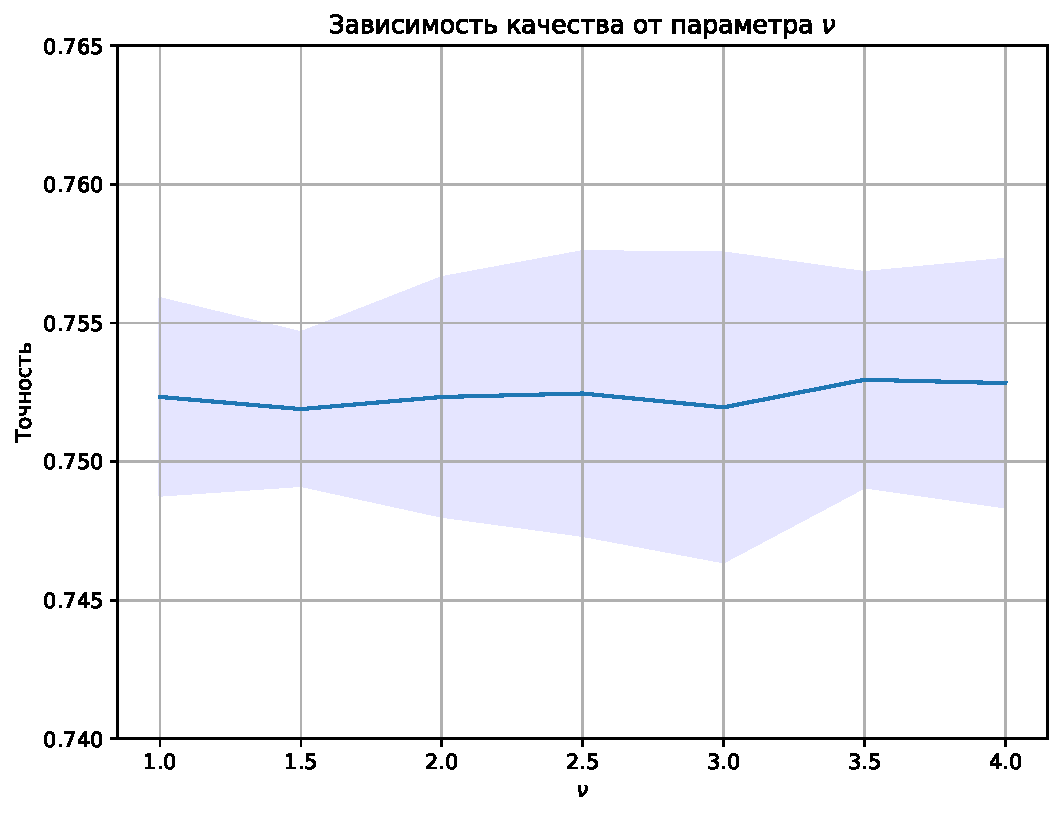
\includegraphics[width=10cm]{nu_ablation.pdf}
    \caption{Зависимость итогового качества от параметра метода $\nu$}
    \label{fig:nu}
\end{figure}
\par

Видим, что с ростом параметра доли $\nu$ увеличивается среднее качество, но при этом растет и среднеквадратичное отклонение (рис. \ref{fig:nu}). Это закономерно, так как большее число кандидатов получается с помощью скрещивания и мутации, а значит в метод вносится дополнительная случайность.

Рассмотрим параметр квантиля значений гиперпараметров $\chi$.

\begin{figure}[h]
    \centering
    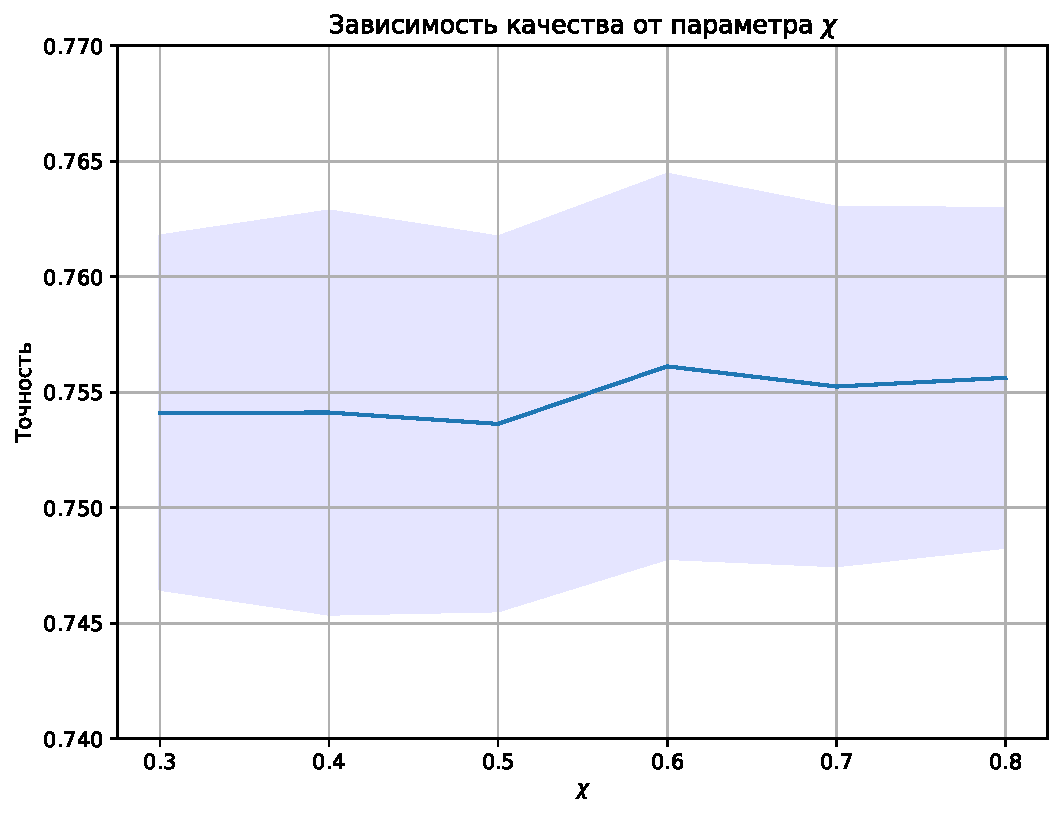
\includegraphics[width=10cm]{chi_ablation.pdf}
    \caption{Зависимость итогового качества от параметра метода $\chi$}
    \label{fig:chi}
\end{figure}
\par

Видим, что с ростом квантиля $\chi$ среднее качество достигает максимума при значении 0.6, а среднеквадратичное отклонение монотонно уменьшается (рис. \ref{fig:chi}). Это происходит из-за того, что для настройки оценок плотностей используются только лучшие значения параметров, а значит уменьшается случайность при мутации. При значении 0.6 достигается компромисс между переиспользованием результатов и случайностью сэмплирования.



\section{Выводы}
Предложенный метод показывает лучшее качество при оптимизации случайного леса и градиентного бустинга с высоким бюджетом вычислений. При малом бюджете и для метода опорных векторов лучше себя показали эволюционный алгоритм и TPE. Объединение идей HyperBand и эволюционных алгоритмов позволило использовать преимущества обоих алгоритмов и преодолеть их слабые стороны.

Модификация мутации позволяет предложенному методу достичь лучшего качества благодаря переходу от полной случайности в изменении параметров к контролируемой случайности в сторону более перспективных значений гиперпараметров. На отложенной тестовой выборке улучшение не так однозначно, но при использовании наборов данных большего объема разница между кросс-валидацией и отложенной выборкой была бы меньше.

Предложенный метод работает хуже, чем эволюционные алгоритмы или TPE в задачах, в которых вычислительный бюджет мал. Это связано с тем, что размеры популяций на итерациях HyperBand становятся слишком малы и метод начинает сильнее полагаться на меньшее число наборов с лучшим качеством при скрещивании.

Дальнейшими направлениями исследования могут быть изучение возможности изменения принципов скрещивания для учета значений оптимизируемой функции, более сложная модификация мутации, учитывающая связи между параметрами и сэмплирование из неисследованных участков пространства гиперпараметров.


\section{Часть 2}
В данной части рассматривается метод DEHB, работающий с непрерывными гиперпараметрами [20]. Предлагается модификация метода, проводятся эксперименты для сравнения результатов работы модифицированного метода и базового.

\section{Алгоритм DEHB}
В алгоритме DEHB сэмплирование из равномерного распределения производится один раз – сэмплируются выборки кандидатов для каждого уровня бюджета вычислений, далее лучшие кандидаты на каждом уровне бюджета сохраняются и передаются в следующие запуски SH. На каждом шаге SH производится модифицированная дифференциальная эволюция – текущие кандидаты, полученные из предыдущего запуска SH, скрещиваются с мутантами, полученными с помощью сэмплирования лучших кандидатов с предыдущей итерации текущего запуска SH [21].

\section{Предлагаемая модификация метода DEHB}
У алгоритма DEHB есть недостаток – он использует случайное сэмплирование всего один раз, и далее кандидаты меняются только за счет дифференциальной эволюции. Алгоритм часто застревает в локальном минимуме и выходит на плато (область примерного постоянства) по значению функции ошибок, что может быть связано с жадным переиспользованием кандидатов, лежащих на маленьком расстоянии друг от друга и имеющим близкие значения функции потерь.
Чтобы этого избежать, предлагается добавлять шумовые векторы к векторам-«мутантам» при эволюции. Благодаря шумовым векторам увеличится широта перебора зависимости функции потерь от гиперпараметров. Это приводит к тому, что некоторые наборы гиперпараметров из популяций будут находиться вне локального минимума. При скрещивании с наборами вне локального минимума DEHB сможет найти новые оптимальные решения.
DEHB создает вектор-``мутант'' по следующей формуле: $v_{i, g} = x_{r_1, g} + F(x_{r_2, g} - x_{r_3, g})$, где $r_1, r_2, r_3$ -- случайные кандидаты из текущей популяции, $F$ -- множитель, равный $0.5$.
Предлагается находить вектор-``мутант'' по модифицированной формуле $v_{i, g} = x_{r_1, g} + F(x_{r_2, g} - x_{r_3, g}) + m(t)\varepsilon$, где $m(t): \mathbb{R} \to \mathbb{R}$ – множитель при шумовом векторе. $m(t)$ может выбираться константой либо зависеть от номера итерации t и уменьшаться со временем, смещая поведение оптимизатора от исследования (exploration) к использованию (exploitation). Также он может зависеть от динамических условий оптимизации – например, увеличиваться после выхода на плато, что препятствует застреванию процесса оптимизации в локальном минимуме. Тщательный выбор функции $m(t)$ обеспечивает наилучшую производительность модифицированного метода оптимизации.

Зададим $m(t)$ следующим образом: 
$$
m(t) = \begin{cases}
			b + s, & \text{если модель находится на плато по ошибке}\\
            b, & \text{иначе}
		 \end{cases},$$ 
где $b$ -- базовое значение шума, $s$ -- шаг шума (параметры метода). Выход на плато определяется отсутствием улучшения качества в течение 10 итераций.

\section{Результаты экспериментов}
В качестве модели для оптимизации гиперпараметров взяты RandomForestClassifier и RandomForestRegressor из библиотеки scikit-learn. Параметры  $b=0,s=0.1$. При увеличении параметра b шум добавляется слишком рано, и это уменьшает стабильность оптимизации. Большие значения параметра s также уменьшают стабильность, но иногда позволяют достичь лучшего качества моделей. Рассматривались следующие гиперпараметры для обоих алгоритмов:
\begin{itemize}
\item Доля признаков $\in [0.1, 0.9]$
\item Минимальное количество объектов для разбиения $\in [2, 128]$
\item Минимальное количество объектов в листе дерева $\in [1, 64]$
\end{itemize}

На графиках линиями изображены средние значения функции ошибки на валидационной выборке для итерации обучения на наборе гиперпараметров. Прозрачные области поверх линий – среднеквадратичное отклонение ошибки. По осям x – количество запусков дифференциальной эволюции для каждой популяции. Функции ошибки: 1-accuracy для классификации и MSE для регрессии.
Метод тестируется на данных из библиотеки scikit-learn  и наборах данных с сайта open-ml (таб. \ref{tab:dehb_datasets}) [16, 19]:
\begin{table}[H]
\centering
\begin{tabular}{|l|l|l|}
\hline
Название           & Тип           & Описание                     \\ \hline
steel-plates-fault & Классификация & Брак стальных пластин        \\ \hline
ilpd               & Классификация & Детекция пациентов           \\ \hline
scene              & Классификация & Предсказание городcкой среды \\ \hline
spambase           & Классификация & Детекция спама               \\ \hline
California Housing & Регрессия     & Стоимость недвижимости       \\ \hline
\end{tabular}
\caption{Наборы данных}
\label{tab:dehb_datasets}
\end{table}

\newpage
 
\begin{figure}[h]
    \centering
    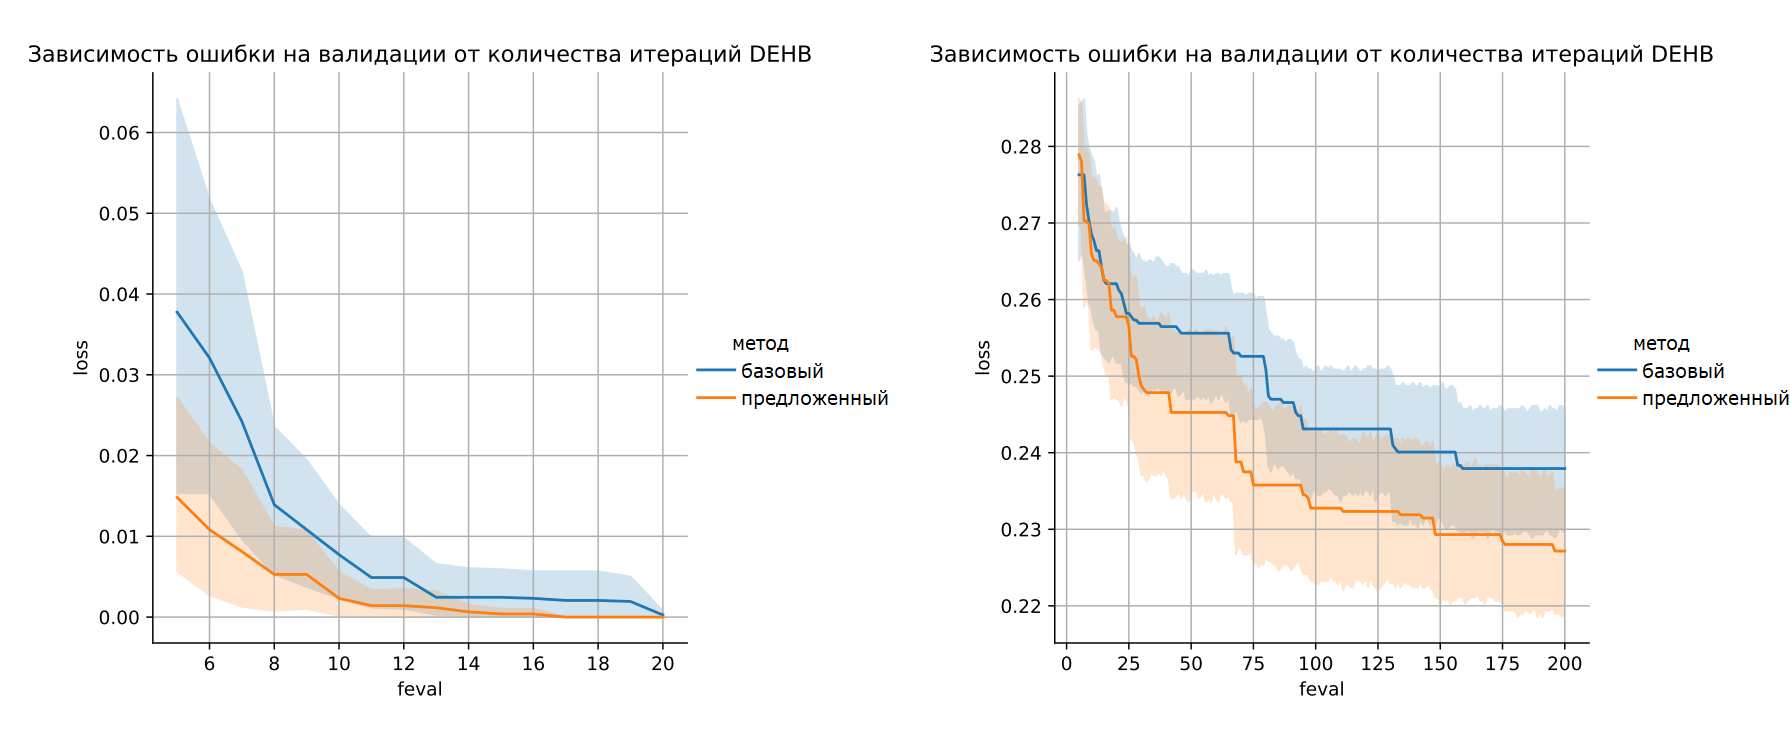
\includegraphics[width=12cm]{exp1.png}
    \caption{Зависимость минимизируемой функции от номера итерации для задачи распознавания брака стальных пластин и задачи распознавания пациентов}
    \label{fig:exp1}
\end{figure}
\par

Видим, что в задаче распознавания брака стальных пластин и в задаче распознавания пациентов с заболеваниями печени предложенный метод стабильно предсказывает лучшие наборы гиперпараметров, чем базовая стратегия мутации (рис. \ref{fig:exp1}). Кроме того, даже несмотря на усреднение ошибок по различным запускам, невооруженным взглядом видно, что базовый метод без зашумления дольше выходит с каждого плато (“ступеньки” на синем графике длиннее).

 
\begin{figure}[h]
    \centering
    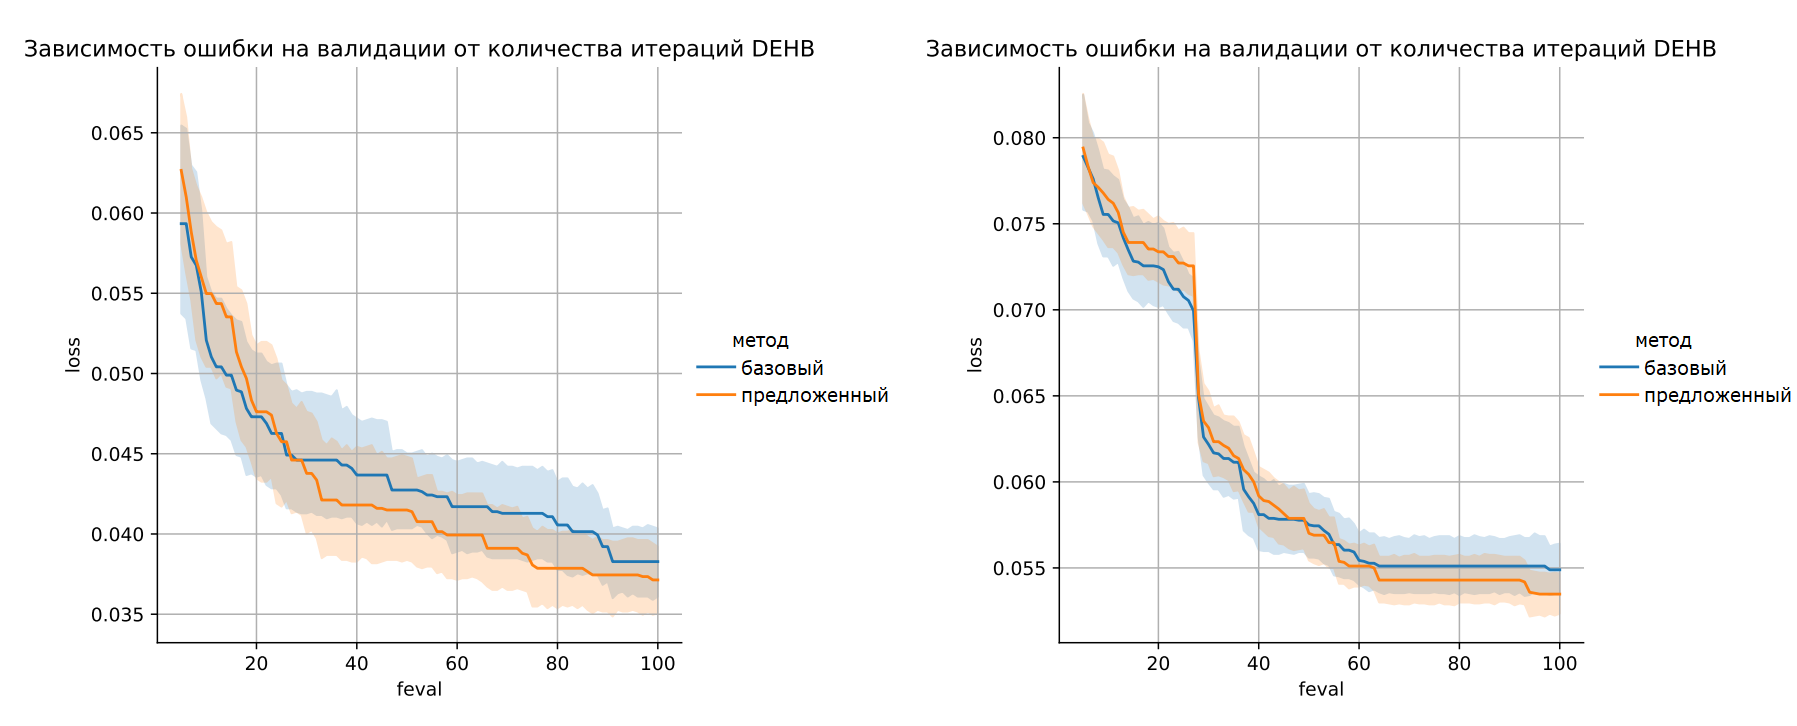
\includegraphics[width=12cm]{exp2.png}
    \caption{Задача предсказания городской среды  и задача распознавания спама}
    \label{fig:exp2}
\end{figure}
\par
При тестировании метода на задаче предсказания городcкой среды по векторным представлениям картинки и задаче распознавания спама метод показывает менее стабильный прирост качества, однако можно заметить, что предложенный метод выходит с плато быстрее классического (рис. \ref{fig:exp2}).

\newpage
Сводные таблицы итоговых ошибок и их среднеквадратичных отклонений в методах приведены ниже:

\begin{table}[h]
\centering
\begin{tabular}{|l|l|l|l|}
\hline
Модель/Данные & 1                & 2                & 3                \\ \hline
DEHB           & $0.001\pm0.005$	& $\mathbf{0.242\pm0.012}$	& $0.038\pm0.006$	\\ \hline
Предложенный       & $\mathbf{0.001\pm0.001}$	& $0.234\pm0.014$	& $\mathbf{0.035\pm0.006}$	\\ \hline
\end{tabular}
\caption{Результаты экспериментов}
\label{tab:dehbrf1}
\end{table}

\begin{table}[h]
\centering
\begin{tabular}{|l|l|l|}
\hline
Модель/Данные  & 4               & 5                \\ \hline
DEHB           & $0.054\pm0.005$	& $0.553\pm0.092$  \\ \hline
Предложенный       	& $\mathbf{0.051\pm0.005}$	& $\mathbf{0.542\pm0.081}$ \\ \hline
\end{tabular}
\caption{Результаты экспериментов}
\label{tab:dehbrf2}
\end{table}

Видим, что предложенный метод показывает улучшение на большинстве задач (таб. \ref{tab:dehbrf1}, таб. \ref{tab:dehbrf2}).
Также стоит заметить, что параметры метода стоит подбирать в зависимости от размерности пространства гиперпараметров, так как шум одной и той же величины с увеличением размерности будет вносить больший вклад в мутацию.

\section{Выводы}
В работе рассматривалась задача автоматической настройки конфигурации моделей машинного обучения, задаваемой вектором гиперпараметров. Была предложена модификация операции мутации при генерации новых конфигураций гиперпараметров в базовом алгоритме DEHB за счет добавления дополнительного шума с изменяемой дисперсией в зависимости от выхода оптимизируемой функции на стабильный уровень значений (плато). Результаты экспериментов показали, что метод показывает улучшение сходимости и нахождение оптимума лучшего качества на большинстве задач. Добавление шума при выходе на плато позволяет получить новых кандидатов и продолжить подбор гиперпараметров с помощью дифференциальной эволюции.

\section{Результаты работы}
Метод, предложенный в первой части работы, позволяет находить оптимальные значения гиперпараметров в задачах с большим бюджетом вычислений. В среднем он работает лучше HyperBand и базового эволюционного алгоритма. Исследована зависимость результатов работы предложенного метода от новых параметров.

Во второй части работы предложена модификация DEHB, исправляющая застревание метода в локальных минимумах функции ошибок. Также исследована зависимость результатов работы от введенных параметров. Вторая часть работы представлена на конференции ИТиММ-2024 в РЭУ имени Г.В. Плеханова в рамках доклада на секции 2: ``Рандомизация поиска гиперпараметров в методе DEHB'', Абрамов В.А, Китов В.В.

\newpage
\section{Список литературы}
\begin{enumerate}
\item Bergstra J., Bengio Y. Random search for hyper-parameter optimization //Journal of machine learning research. – 2012. – Т. 13. – №. 2.

\item Bischl B. et al. Hyperparameter optimization: Foundations, algorithms, best practices, and open challenges //Wiley Interdisciplinary Reviews: Data Mining and Knowledge Discovery. – 2023. – Т. 13. – №. 2. – С. e1484.

\item Awad N., Mallik N., Hutter F. Dehb: Evolutionary hyperband for scalable, robust and efficient hyperparameter optimization //arXiv preprint arXiv:2105.09821. – 2021.

\item Talbi E. G. Optimization of deep neural networks: a survey and unified taxonomy. – 2020.

\item Hutter F., Hoos H. H., Leyton-Brown K. Sequential model-based optimization for general algorithm configuration //Learning and Intelligent Optimization: 5th International Conference, LION 5, Rome, Italy, January 17-21, 2011. Selected Papers 5. – Springer Berlin Heidelberg, 2011. – С. 507-523.

\item Wistuba M., Schilling N., Schmidt-Thieme L. Scalable gaussian process-based transfer surrogates for hyperparameter optimization //Machine Learning. – 2018. – Т. 107. – №. 1. – С. 43-78.

\item Bergstra J. et al. Algorithms for hyper-parameter optimization //Advances in neural information processing systems. – 2011. – Т. 24.

\item Lindauer M. et al. SMAC3: A versatile Bayesian optimization package for hyperparameter optimization //Journal of Machine Learning Research. – 2022. – Т. 23. – №. 54. – С. 1-9.

\item Schilling N., Wistuba M., Schmidt-Thieme L. Scalable hyperparameter optimization with products of gaussian process experts //Machine Learning and Knowledge Discovery in Databases: European Conference, ECML PKDD 2016, Riva del Garda, Italy, September 19-23, 2016, Proceedings, Part I 16. – Springer International Publishing, 2016. – С. 33-48.

\item Young S. R. et al. Optimizing deep learning hyper-parameters through an evolutionary algorithm //Proceedings of the workshop on machine learning in high-performance computing environments. – 2015. – С. 1-5.

\item Alibrahim H., Ludwig S. A. Hyperparameter optimization: Comparing genetic algorithm against grid search and bayesian optimization //2021 IEEE Congress on Evolutionary Computation (CEC). – IEEE, 2021. – С. 1551-1559.

\item Jamieson K., Talwalkar A. Non-stochastic best arm identification and hyperparameter optimization //Artificial intelligence and statistics. – PMLR, 2016. – С. 240-248.

\item Li L. et al. Hyperband: A novel bandit-based approach to hyperparameter optimization //Journal of Machine Learning Research. – 2018. – Т. 18. – №. 185. – С. 1-52.

\item Falkner S., Klein A., Hutter F. BOHB: Robust and efficient hyperparameter optimization at scale //International conference on machine learning. – PMLR, 2018. – С. 1437-1446.

\item Scott D. W. Multivariate density estimation: theory, practice, and visualization. – John Wiley \& Sons, 2015.

\item Pedregosa F. et al. Scikit-learn: Machine learning in Python //the Journal of machine Learning research. – 2011. – Т. 12. – С. 2825-2830.

\item Akiba T. et al. Optuna: A next-generation hyperparameter optimization framework //Proceedings of the 25th ACM SIGKDD international conference on knowledge discovery \& data mining. – 2019. – С. 2623-2631.

\item Ke G. et al. Lightgbm: A highly efficient gradient boosting decision tree //Advances in neural information processing systems. – 2017. – Т. 30.

\item Vanschoren J. et al. OpenML: networked science in machine learning //ACM SIGKDD Explorations Newsletter. – 2014. – Т. 15. – №. 2. – С. 49-60.

\item Awad N., Mallik N., Hutter F. Dehb: Evolutionary hyperband for scalable, robust and efficient hyperparameter optimization //arXiv preprint arXiv:2105.09821. – 2021.

\item Storn R., Price K. Differential evolution–a simple and efficient heuristic for global optimization over continuous spaces //Journal of global optimization. – 1997. – Т. 11. – С. 341-359.

\end{enumerate}


\newpage
\section{Приложение}
Значения качества на отложенных тестовых выборках для всех задач.

Случайный лес в задачах регрессии:
\begin{table}[h]
\centering
\begin{tabular}{|l|l|l|l|}
\hline
Алгоритм        & space\_ga                     & topo\_2\_1            & us\_crime                     \\ \hline
HyperBand       & $0.0144 \pm 0.0003$          & $0.0008 \pm 0.0000$ & $0.0177 \pm 0.0001$          \\ \hline
Эволюция        & $0.0149 \pm 0.0006$          & $0.0008 \pm 0.0000$ & $\mathbf{0.0176 \pm 0.0001}$ \\ \hline
EvoHyperBand    & $0.0148 \pm 0.0006$          & $0.0008 \pm 0.0000$ & $\mathbf{0.0176 \pm 0.0001}$ \\ \hline
EvoHyperBandMut & $\mathbf{0.0143 \pm 0.0000}$ & $0.0008 \pm 0.0000$ & $\mathbf{0.0176 \pm 0.0001}$ \\ \hline
TPE             & $0.0146 \pm 0.0001$          & $0.0008 \pm 0.0000$ & $0.0177 \pm 0.0001$          \\ \hline
\end{tabular}
\caption{MSE случайного леса на отложенной выборке (задача регрессии)}
\label{tab:rf_regr_test}
\end{table}

Метод опорных векторов в задачах классификации:
\begin{table}[h]
\centering
\begin{tabular}{|l|l|l|l|}
\hline
Алгоритм        & ilpd              & blood             & kr-kp             \\ \hline
HyperBand       & $0.6735 \pm 0.1331$ & $0.7487 \pm 0.0291$ & $0.8589 \pm 0.0800$ \\ \hline
Эволюция        & $0.7299 \pm 0.0134$ & $0.7793 \pm 0.0020$ & $0.9556 \pm 0.0069$ \\ \hline
EvoHyperBand    & $0.7034 \pm 0.1243$ & $0.7567 \pm 0.0316$ & $0.9352 \pm 0.0232$ \\ \hline
EvoHyperBandMut & $0.6427 \pm 0.1708$ & $0.7667 \pm 0.0119$ & $0.9334 \pm 0.0333$ \\ \hline
TPE             & $\mathbf{0.7350 \pm 0.0000}$ & $\mathbf{0.7800 \pm 0.0000}$ & $\mathbf{0.9609 \pm 0.0000}$ \\ \hline
\end{tabular}
\caption{Точность метода опорных векторов на отложенной выборке (задача классификации)}
\label{tab:svm_test}
\end{table}

\newpage

Градиентный бустинг с бюджетом 243 в задачах классификации:
\begin{table}[h]
\centering
\begin{tabular}{|l|l|l|l|}
\hline
Алгоритм        & credit-g          & ilpd              & kr-kp             \\ \hline
HyperBand       & $0.7740 \pm 0.0097$ & $0.7487 \pm 0.0214$ & $\mathbf{0.9747 \pm 0.0072}$ \\ \hline
Эволюция        & $0.7700 \pm 0.0143$ & $\mathbf{0.7530 \pm 0.0150}$ & $0.9716 \pm 0.0069$ \\ \hline
EvoHyperBand    & $0.7605 \pm 0.0157$ & $0.7462 \pm 0.0094$ & $0.9745 \pm 0.0053$ \\ \hline
EvoHyperBandMut & $0.7600 \pm 0.0116$ & $0.7496 \pm 0.0195$ & $0.9745 \pm 0.0063$ \\ \hline
TPE             & $\mathbf{0.7880 \pm 0.0040}$ & $0.7436 \pm 0.0000$ & $\mathbf{0.9747 \pm 0.0015}$ \\ \hline
\end{tabular}
\caption{Точность градиентного бустинга на отложенной выборке (задача классификации)}
\label{tab:boosting_test}
\end{table}


Градиентный бустинг с бюджетом 500 в задачах регрессии:
\begin{table}[h]
\centering
\begin{tabular}{|l|l|l|l|}
\hline
Алгоритм        & space\_ga          & topo\_2\_1            & us\_crime          \\ \hline
HyperBand       & $0.0113 \pm 0.0003$ & $0.0008 \pm 0.0000$ & $0.0175 \pm 0.0003$ \\ \hline
Эволюция        & $\mathbf{0.0111 \pm 0.0004}$ & $0.0008 \pm 0.0000$ & $0.0174 \pm 0.0003$ \\ \hline
EvoHyperBand    & $0.0112 \pm 0.0003$ & $0.0008 \pm 0.0000$ & $0.0175 \pm 0.0004$ \\ \hline
EvoHyperBandMut & $0.0115 \pm 0.0004$ & $0.0008 \pm 0.0000$ & $\mathbf{0.0172 \pm 0.0007}$ \\ \hline
TPE             & $0.0115 \pm 0.0000$ & $0.0008 \pm 0.0000$ & $0.0176 \pm 0.0000$ \\ \hline
\end{tabular}
\caption{MSE градиентного бустинга на отложенной выборке (задача регрессии)}
\label{tab:boosting_regr_test}
\end{table}

\end{document}